\documentclass[border=10pt]{standalone}

\usepackage{tikz}
\usepackage{tikzsymbols}
\usetikzlibrary{calc,patterns,shapes.geometric}

\def\centerarc[#1](#2)(#3:#4:#5){\draw[#1] ($(#2)+({#5*cos(#3)},{#5*sin(#3)})$) arc (#3:#4:#5);}

\begin{document}
	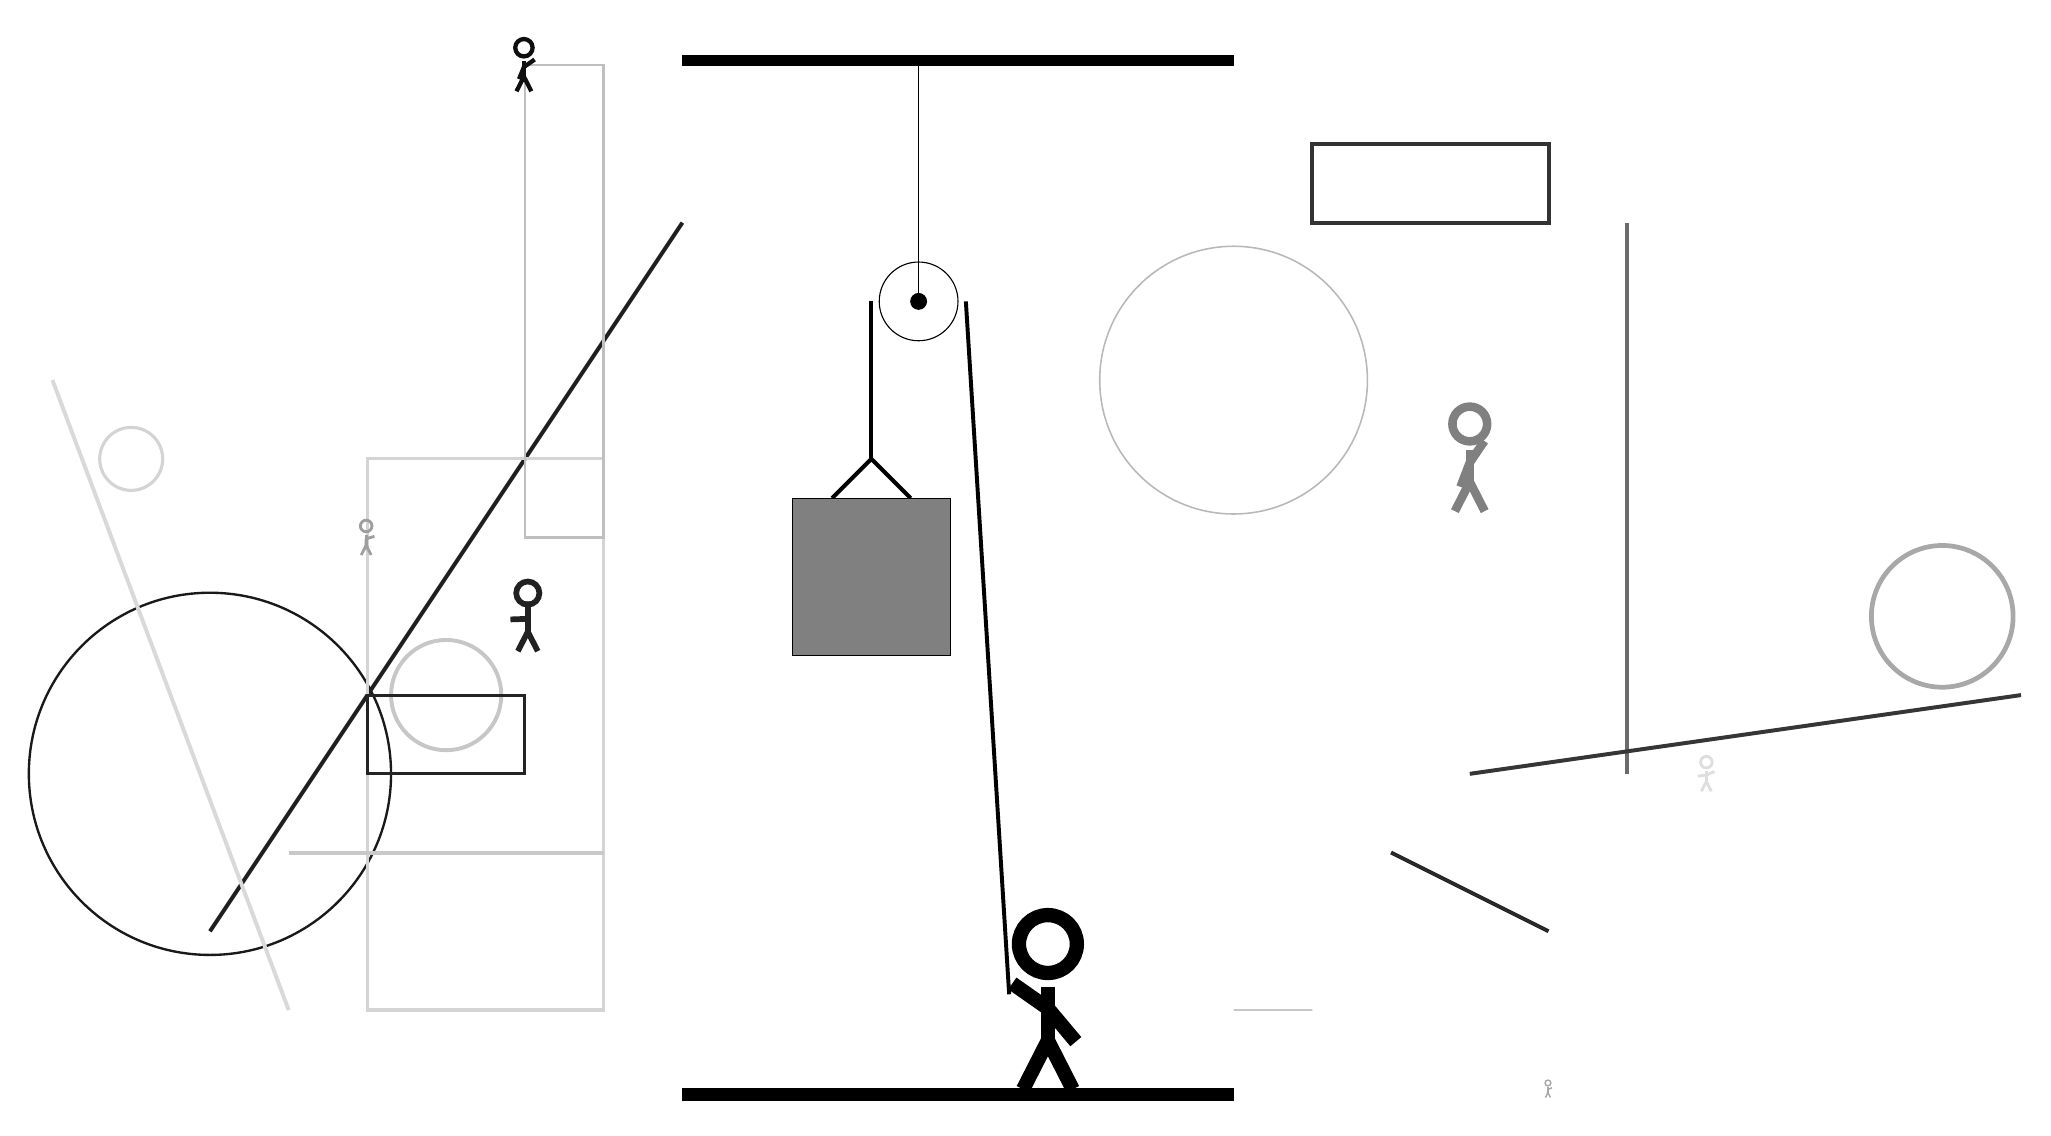
\begin{tikzpicture}
		%%%%% START %%%%%
		
		\draw[fill=black] (-2, 10) rectangle (5, 10.125);
		
		\draw (1, 7) circle (0.5);
		\draw[fill=black] (1, 7) circle (0.1);
		\draw (1, 10) -- (1, 7);
		
		\draw[line width=0.5mm] (-0.1, 4.5) -- (0.4, 5.0) -- (0.9, 4.5);
		\draw[fill=black!50] (-0.6, 4.5) rectangle (1.4, 2.5);
		
		\draw [line width=0.3mm, color=black!90](-8, 1) circle (2.3);
		
		\draw[line width=0.3mm, color=black!22] (6, -2) rectangle (5, -2);
		\draw[line width=0.5mm, color=black!80] (6, 9) rectangle (9, 8);
		\draw[line width=0.5mm, color=black!88](-2, 8) -- (-8, -1);
		\draw [line width=0.5mm, color=black!22](-5, 2) circle (0.7);
		\draw[line width=0.4mm, color=black!17] (-3, -2) rectangle (-6, 5);
		\draw[line width=0.5mm, color=black!15](-7, -2) -- (-10, 6);
		\draw [line width=0.6mm, color=black!34](14, 3) circle (0.9);
		\node[line width=0.4mm, color=black!38] at (-6, 4) {\Strichmaxerl[2][89][17]};
		\draw [line width=0.2mm, color=black!28](5, 6) circle (1.7);
		
		\node[line width=0.2mm, color=black!13] at (11, 1) {\Strichmaxerl[2][7][24]};
		\draw[line width=0.4mm, color=black!86] (-4, 2) rectangle (-6, 1);
		\draw[line width=0.3mm, color=black!25] (-3, 10) rectangle (-4, 4);
		\draw[line width=0.5mm, color=black!21](-3, 0) -- (-7, 0);
		\draw [line width=0.4mm, color=black!17](-9, 5) circle (0.4);
		\node[line width=0.2mm, color=black!50] at (8, 5) {\Strichmaxerl[6][69][56]};
		
		\draw[line width=0.5mm, color=black!58](10, 1) -- (10, 8);
		\draw[line width=0.5mm, color=black!84](9, -1) -- (7, 0);
		\draw[line width=0.5mm, color=black!79](8, 1) -- (15, 2);
		\node[line width=0.7mm, color=black!94] at (-4, 10) {\Strichmaxerl[3][68][35]};
		\node[line width=0.7mm, color=black!35] at (9, -3) {\Strichmaxerl[1][83][22]};
		\node[line width=0.6mm, color=black!87] at (-4, 3) {\Strichmaxerl[4][2][89]};
		
		\draw[line width=0.5mm] (0.4, 7) -- (0.4, 5.0);
		\centerarc[line width=0.5mm](1, 7)(0:180:0.6);
		\draw[line width=0.5mm](1.6, 7) -- (2.15, -1.8);
		
		\node at (2.6, -1.9) {\Strichmaxerl[10][-35][-50]};
		
		\draw[fill=black] (-2, -3) rectangle (5, -3.15);
		
		%%%%% END %%%%%
	\end{tikzpicture}
\end{document}